%!TEX TS-program = xelatex
\documentclass[12pt, a4paper]{article}  

%%%%%%%%%% Математика %%%%%%%%%%
\usepackage{amsmath,amsfonts,amssymb,amsthm,mathtools} 
%\mathtoolsset{showonlyrefs=true}  % Показывать номера только у тех формул, на которые есть \eqref{} в тексте.
%\usepackage{leqno} % Нумерация формул слева

 
%%%%%%%%%%%%%%% Шрифты %%%%%%%%%%%

\usepackage[british,russian]{babel} % выбор языка для документа
\usepackage[utf8]{inputenc} % задание utf8 кодировки исходного tex файла

\usepackage{fontspec}         % пакет для подгрузки шрифтов
\setmainfont{Arial}   % задаёт основной шрифт документа


\usepackage{unicode-math}     % пакет для установки математического шрифта
% шрифт для математики
\setmathfont{Asana-Math.otf}
\usepackage{graphicx}                  % Для вставки рисунков
\usepackage{graphics}
\usepackage{wrapfig}
\usepackage{caption}


\graphicspath{{images/}}



%%%%%%%%%%%%%%%%%%%%%%%% Оформление %%%%%%%%%%%%%%%%%%%%%%%%%%%%%%%%%

\usepackage[paper=a4paper,top=15mm, bottom=15mm,left=35mm,right=10mm,includefoot]{geometry}
\usepackage{indentfirst}       % установка отступа в первом абзаце главы


% Заголовок
\author{Спиридонов Роман}
\title{Домашнее задание №2. Упражнение 3.}
\date{\today}

\begin{document}

\maketitle
	Сразу  хочу сказать, что текст писал не я. Мне было лень, поэтому я попросил подругу. Это не я такой романтичный.
\section{Упражнение 3 (Где деньги, Лебовски?)}	



\Large{\fontspec{Harry Potter (Russian Version of Gfdtk)}{Гермионе Грейнджер}
	\vspace{0.3cm}
	%0.171 4 3
	
	\begin{wrapfigure}{l}{0.2\linewidth}
		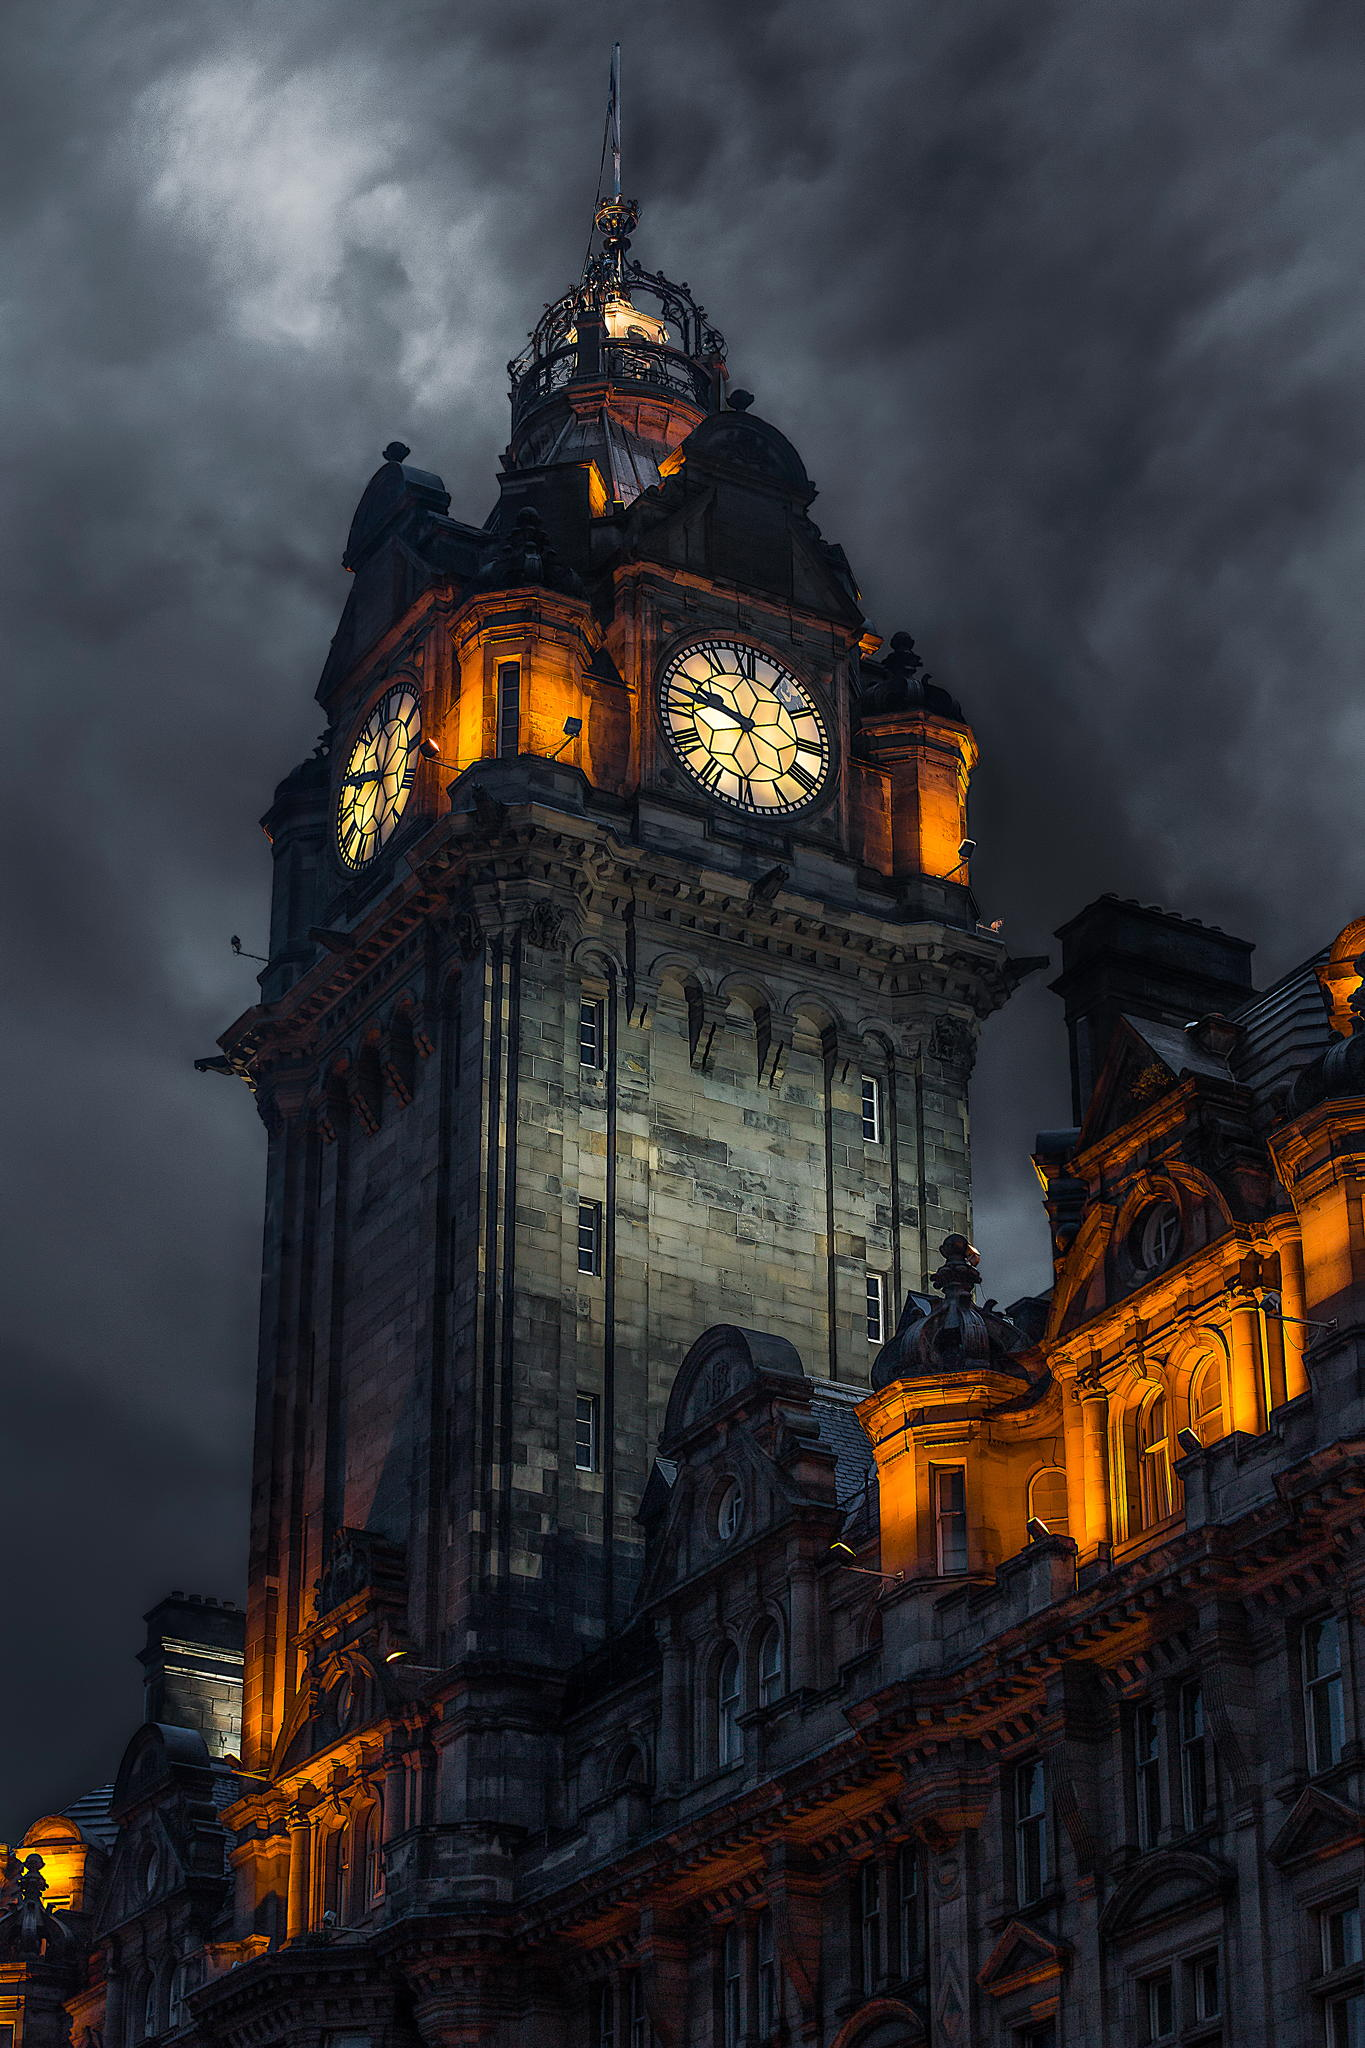
\includegraphics[height=6cm,width=3.5cm]{tower.jpg}
	\end{wrapfigure}
	
	
\Large{\fontspec{Harry Potter (Russian Version of Gfdtk)}{
Дорогая Гермиона, я не свожу с тебя глаз ровно с того дня, как увидел тебя на платформе Лондона в далеком 2010. У тебя были такие забавные веснушки, а твой смех заставлял улыбаться даже незнакомых людей. Я был счастлив, когда распределяющая шляпа отправила меня в Гриффиндор, ведь это означало, что следующие 5 лет мы будем каждый день находиться рядом.

Меня часто смешит твой слишком серьезный подход ко всему, что ты делаешь, но одновременно меня это восхищает. Время пролетело так быстро... Я не успел заметить, как из той забавной девчушки ты выросла в красивую, не по годам умную девушку. И вот когда времени у меня осталось так мало (ведь через пол года мы заканчиваем школу и разъезжаемся), я решил сказать тебе то, что должен был очень давно. Я люблю тебя и восхищаюсь тобой, Гермиона Грейнджер. Ты удивительный человек и замечательный друг. Прости, что никогда не говорил тебе это раньше.

Сегодня в 19:00 я с нетерпением буду ждать тебя под башней с часами, не опаздывай.}}
\begin{flushright}
	От\\
	Рона Уизли
\end{flushright}
	
\end{document}